\chapter{関連研究}
関連研究や用語の定義,先行研究及びアプリケーションの先行事例を示す.

\section{時間の定義}
時間は出来事や変化を認識する為の基礎的概念の一つであり,芸術,哲学,自然科学,心理学を始めとした諸分野で議論されているテーマである.時間管理の定義は表~\ref{tb:Lakein}に示したLakeinの定義[]をはじめとして様々である[].

\begin{table}[htb]
\begin{center}
  \begin{tabular}{|l|l|} \hline
   1 & すべきことを決定する \\ \hline
   2 & 達成するための目標を設定する \\ \hline
   3 & 優先順位を決める \\ \hline
   4 & 取り組む課題のプランニングを作る \\ \hline
  \end{tabular}
  \caption{Lakeinによる時間管理の定義}
  \label{tb:Lakein}
\end{center}
\end{table}

Claessens et al. (2007)は,先行研究の定義を俯瞰した上で,時間管理を"目標を達成するために時間を効果的に使用する行動"と定義し時間管理の行動を更に以下の3つに分類した[](~\ref{tb:Claessens}参照).

\begin{table}[htb]
\begin{center}
  \begin{tabular}{|l|l|} \hline
   時間アセスメント行動(time assessment behavior): \\ ~~~過去,現在,未来の時間を認識し,時間の使い方に関して認識する事 \\ \hline
   プランニング行動(planning behavior): \\  ~~~時間を効率的に使用する事を目的とする事 \\ \hline
   モニタリング行動(monitoring behavior): \\ ~~~行動中における時間の配分のモニタリング・不測の事態へのリスクヘッジ等 \\ \hline
  \end{tabular}
  \caption{Claessens et al. による時間管理の定義}
  \label{tb:Claessens}
\end{center}
\end{table}

\section{先行研究について}
時間管理研究は大きく分けて時間管理がもたらす効果の研究\footnote{時間管理がもたらす効果の研究は主にa. 時間管理と他の指標の相関関係を調べる研究,b. 時間管理のプロセスモデルの研究 c. 時間管理トレーニングの研究の3タイプに分類が可能である.}と時間管理能力の研究がある.時間管理能力の研究では必要時間の正確な見積もりの能力に関する研究である.見積もり時間は与えられた課題の時間 (Roy, Mitten, \&Christenfeld, 2008)や経験の有無(Roy\&Christenfeld, 2007)によって左右されるものの,一般的には課題の見積もりを少なく見積もる傾向があるとされている(Roy,Mitten, \& Christenfeld, 2008)Kahneman et al. (2004).見積もりが難しい理由としては記憶バイアス (memory bias) すなわち,費やした時間に対する誤った記憶が関連する(e.g. , Roy, Christenf eld, \& McKenzie,2005)と言う考えや,知覚時間の歪み\footnote{例えば心拍数\cite{MatudaHorie2011}\cite{MatudaIchikawa2015},体温\cite{MatudaHorie2011}\cite{Hoagland1933},血圧\cite{MatudaHorie2011}など}が考えられている.こうした見積もり時間のずれに左右される事がない様に適切な見積もりを行うためのフレームワークとしてガントチャートやPERT図が使われる事が多い.

\section{日常生活動作について}
日常生活動作(Activities of Daily Living;ADL)とは,人が日常生活において繰り返す,身の回りの活動や動作のことである.具体的には,身の回りの動作(食事,更衣,整容,排泄,入浴の各動作),移動動作,その他生活関連動作(家事動作,交通機関の利用等)を指す\cite{Sakai2003}.我々は外出準備に平均1時間程度日常生活動作を複数こなしている\cite{duhouse}.本研究では「起床時から外出時刻までに外出準備として行われる日常生活動作」とする.

\section{アプリケーションに関して}
今日日常生活動作を対象にした時間管理に関するiOSアプリケーションが開発されている.例えば,「たすくま」はタスクシュート式\footnote{タスクシュートは大橋悦夫が開発した管理手法であり,1日の仕事を直列に並べ,見積時間を出すと終了時刻を自動予測するシステムを用いて行われる.}のタスク管理アプリである\cite{Taskuma}.「たすくま」はタスク毎の時間を記録すると,予測タスクの自動生成が行われ,日常生活動作を始めとしたルーティンワークの予測が行われる.ルーチンタイマーは複数タスクを「ルーチン」として登録し,設定した所要時間をもとに一つ一つアナウンスされるアプリケーションである\cite{RoutineTimer}.ルーチンタイマーの導入によって対象のルーティンワークの可視化や登録したタスク別終了予定時刻の把握が可能である.

\begin{figure}[ht]
\begin{center}
\begin{tabular}{c}

  	\begin{minipage}[b]{0.5\linewidth}
	\begin{center}
		\fbox{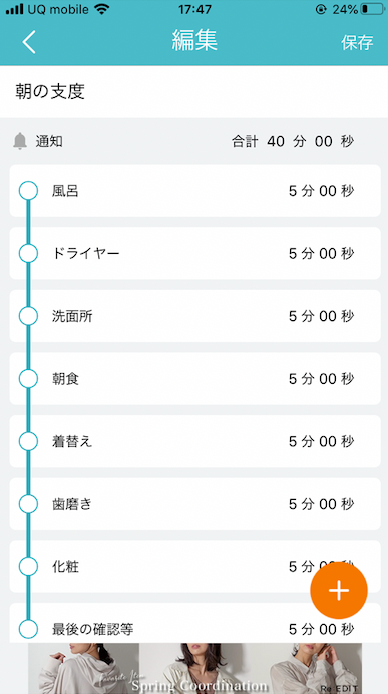
\includegraphics[width=5cm]{images/2/routine1.png}}
		\caption{ルーティンワークカウントダウン}
		\label{fig:goal_alert}
	\end{center}
  	\end{minipage}

  	\begin{minipage}[b]{0.5\linewidth}
	\begin{center}
		\fbox{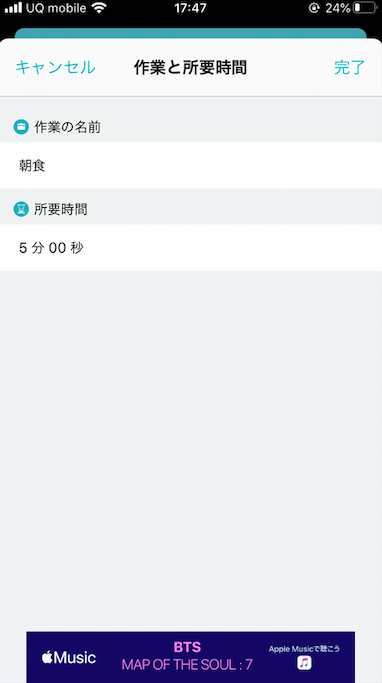
\includegraphics[width=5cm]{images/2/routine2.png}}
		\caption{ルーティンワークカウントダウン}
		\label{fig:top_goal}
	\end{center}
  	\end{minipage}

\end{tabular}
\end{center}
\end{figure}


\section{まとめ}
本章では,本研究における関連研究を整理し,問題意識を洗い出した.
次章では,筆者が本研究に先立ち行った研究について述べ,問題意識を洗い出す.